\documentclass{beamer}
\mode<presentation>{\usetheme{Copenhagen}}

\usepackage[tikz]{bclogo}
\presetkeys{bclogo}{
	ombre=true,
	epBord=3,
	couleur = blue!15!white,
	couleurBord = red,
	arrondi = 0.2,
	logo=\bctrombone
}{}
\usepackage{etoolbox}
\makeatletter
\patchcmd{\insertverticalnavigation}%
{\ifx\beamer@nav@css\beamer@hidetext{\usebeamertemplate{section in sidebar}}\else{\usebeamertemplate{section in sidebar shaded}}\fi}%
{{\usebeamertemplate{section in sidebar}}}{}{}
\makeatother
\title{Machine Learning in Astronomy}
\author{Reza Monadi}
\institute{UC Riverside}
\date{May 14, 2020}
\begin{document}
	
	\frame{\titlepage}
	
	\begin{frame}
	\centering
	
\includegraphics[height=6cm, angle=0,origin=c]{ml.jpg}
	\tiny{credit: 365datascience.com}
	
\end{frame}

	
\section{Questions to be addressed}
\frame{
	\begin{itemize}
		\uncover<1->{\item Is \textbf{ML} the same as \textbf{Statistics}?}
		\uncover<2->{\item How astronomy is tied to \textbf{BIG DATA}?}
		\uncover<3->{\item How to implement \textbf{ML} in astronomy? }
%		\uncover<4->{\item How \textbf{ML} helps \textbf{SKA}?}
		\uncover<4->{\item What are the pitfalls of \textbf{ML}?}
	\end{itemize}
	}

\section{ML overview}\frame{
		\centering
		
		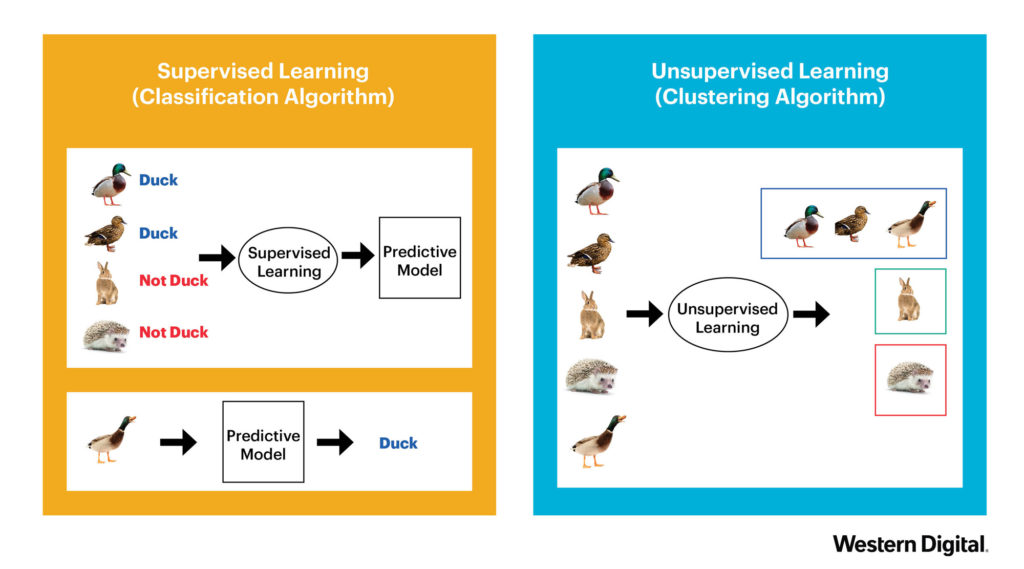
\includegraphics[width=\linewidth]{super.jpg} \\
%		{\tiny{credit: ClickUp (Productivity Platforms)}}
		}
\subsection{Supervised learning}
\frame{
	\frametitle{How supervised learning works?}
	\centering
	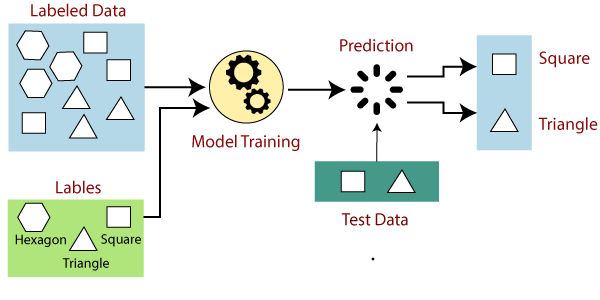
\includegraphics[width=\linewidth]{example-supervised.png}
	{\tiny{credit: javatpoint.com}}
	
}
\frame{ \frametitle{How supervised learning works?}
\begin{itemize}
	\uncover<1->{\item We need a set of measurements. }
	\uncover<2->{\item We need the label for each measurement.}
	\uncover<3->{\item We define a model and let the machine learn from examples.}
	\uncover<4->{\item We ask the machine to predict label of unseen measurements. }
\end{itemize}

\uncover<5->{\begin{bclogo}{Supervised learning vs. model fitting}
		\begin{itemize}
		\uncover<6->{\item Supervised learning: 
			\begin{enumerate}
				\uncover<7->{ \item The model gets adapted by data}
				\uncover<8->{\item Can be very nonlinear and complex}
			\end{enumerate}
					}
		\uncover<9->{\item Traditional model fitting: 
			\begin{enumerate}
				\uncover<10->{\item Model is predefined}
				\uncover<11->{\item Model adaptivity is limited}
			\end{enumerate}}
\end{itemize} \end{bclogo}}	
}
\frame{\frametitle{Stages of Supervised Learning}
	
\begin{itemize}
	\uncover<1->{\item Training: 
		\begin{enumerate}
			\uncover<2->{\item Select a model }
			\uncover<3->{\item Set up hyper-parameters of model}
			\uncover<4->{\item Teach the machine by training set}
		\end{enumerate} }
	\uncover<5->{\item Validation: 
		\begin{enumerate}
			\uncover<6->{\item Change the hyper-parameters  }
			\uncover<7->{\item Select the optimum hyper-parameters}
	\end{enumerate} } 
\uncover<8->{\item Testing: 
	\begin{enumerate}
	\uncover<9->{\item Test learned model by an unseen part of the data-set. }
	\uncover<10->{\item Select the best model and use it for predictions.}
\end{enumerate} } 

\end{itemize}
}
\frame{
	\frametitle{Supervised learning methods in astronomy?}
	
	\begin{itemize}
	\uncover<1->{\item Classification: discrete targets}
		\begin{enumerate}[a]
			\uncover<1->{\item Spectrum: quasar, star, galaxy, supernova, ...}
			\uncover<2->{\item Timing: Binary/isolated pulsar, variability,... }
			\uncover<3->{\item Galaxy morphology: spiral, dwarf, elliptical, ...  }
		\end{enumerate}
	\uncover<1->{\item Regression: continuous targets}
	\begin{enumerate}[a]
		\uncover<1->{\item }
		\uncover<2->{\item Photometry: redshift estimation }
		\uncover<3->{\item }
	\end{enumerate}
	
	\uncover<4->{\item DBSCAN:}
	\uncover<5->{\item :}
	\uncover<6->{\item OPTICS:}
	
\end{itemize}
}
\frame{\frametitle{Deep/Shallow Artificial Neural Networks}}
\frame{\frametitle{}}

\subsection{Unsupervised learning}
\frame {\frametitle{How unsupervised learning works?}}
\frame{\frametitle{Clustering}
\begin{itemize}
	\uncover<1->{\item KMeans:}
	\uncover<2->{\item DBSCAN:}
	\uncover<3->{\item :}
	\uncover<4->{\item OPTICS:}

\end{itemize}
}
\section{Big Data in astronomy}\frame{
\centering
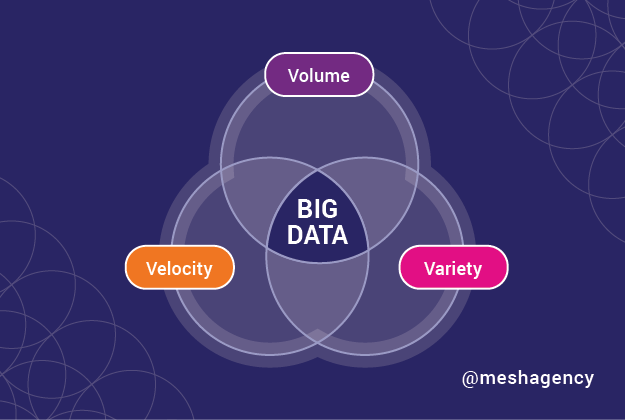
\includegraphics[height=6cm, angle=0,origin=c]{vvv.png}
}
\subsection{Big telescopes}
\frame{
\frametitle{TMT}
}
\frame{
	\frametitle{JWST}
}
%\subsection{Higher resolution}\frame{}
\subsection{Simulations}\frame{}
\subsection{Surveys}
\frame{
	\frametitle{Sloan Digital Sky Server}
}
\frame{
	\frametitle{Zwicky Transient Facility}
}

\frame{
	\frametitle{Gaia}
}
\frame{
	\frametitle{DESI}
}
\frame{
\frametitle{Square Kilometer Array}
}
\section{ML applications in astronomy}\frame{text}
\subsection{a}\frame{}
\subsection{b}\frame{}


\subsection{a}\frame{}
\subsection{b}\frame{}
\section{ML limitations}\frame{text}
\subsection{a}\frame{}
\subsection{b}\frame{}
\end{document}